\documentclass[paper=A4,pagesize=auto,12pt,headinclude=true,footinclude=true,BCOR=0mm,DIV=calc]{scrartcl}
\usepackage[english]{babel}
\usepackage[utf8]{inputenc}
\usepackage{graphicx}
\usepackage{geometry}
\usepackage[T1]{fontenc}
\usepackage{lmodern}
\usepackage{amsmath}
\usepackage[scaled]{uarial}
\usepackage{blindtext}
\usepackage{hyperref}
\usepackage{eurosym}
\usepackage{color}
\usepackage{subfigure}
\usepackage{listings}
\usepackage{float}
\usepackage{amsfonts}
\usepackage{amssymb}
\usepackage{graphics}
\usepackage{wrapfig}
\usepackage{setspace}
\usepackage[font=footnotesize]{caption}
\usepackage[format=plain,
justification=RaggedRight,
singlelinecheck=false]
{caption}
\usepackage{textcomp}
\geometry{
	left=2.5cm,
	right=2.5cm,
	top=2.5cm,
	bottom=2cm,
}
\makeatletter
\newcommand{\MSonehalfspacing}{%
	\setstretch{1.44}%  default
	\ifcase \@ptsize \relax % 10pt
	\setstretch {1.44}%
	\or % 11pt
	\setstretch {1.44}%
	\or % 12pt
	\setstretch {1.44}%
	\fi
}
\MSonehalfspacing
\setlength{\parindent}{0pt}

\begin{document}
	
	\title{Github Repository Classifier\\
		Contribution to the InformatiCup}
	\author{\textbf{Rami Aly$^{1}$, Andre Schurat}$^{2}$\\
		$^{1}$ University of Hamburg\\
		$^{2}$ Technical University of Dortmund}
	\maketitle
	
	\newpage
	
	\newpage
	
	\tableofcontents 
	
	\newpage
	\section{Selecting features} 
	\subsection{General thoughts}
	In the early beginning of our process we discussed our selection of features. We analyzed many repositories and we realized that it is not possible for us to manually enclose the available data sets in a way where we would not miss important features. If we choose for example web sites produced by Jekyell as the indicator for the class WEB we will probably miss other web applications as the software and the use-case market is to wide to manually find all necessary features. So in the first step we decided to maximize the possible information which can be obtained while also gathering statistically irrelevant information. In further context we will call this phenomenon “information noise”.
	\subsection{Selected features}
	The following graphic visualizes the structure behind our selected features.
	
	\begin{figure}[H]
		\subfigure{\label{konfiguration}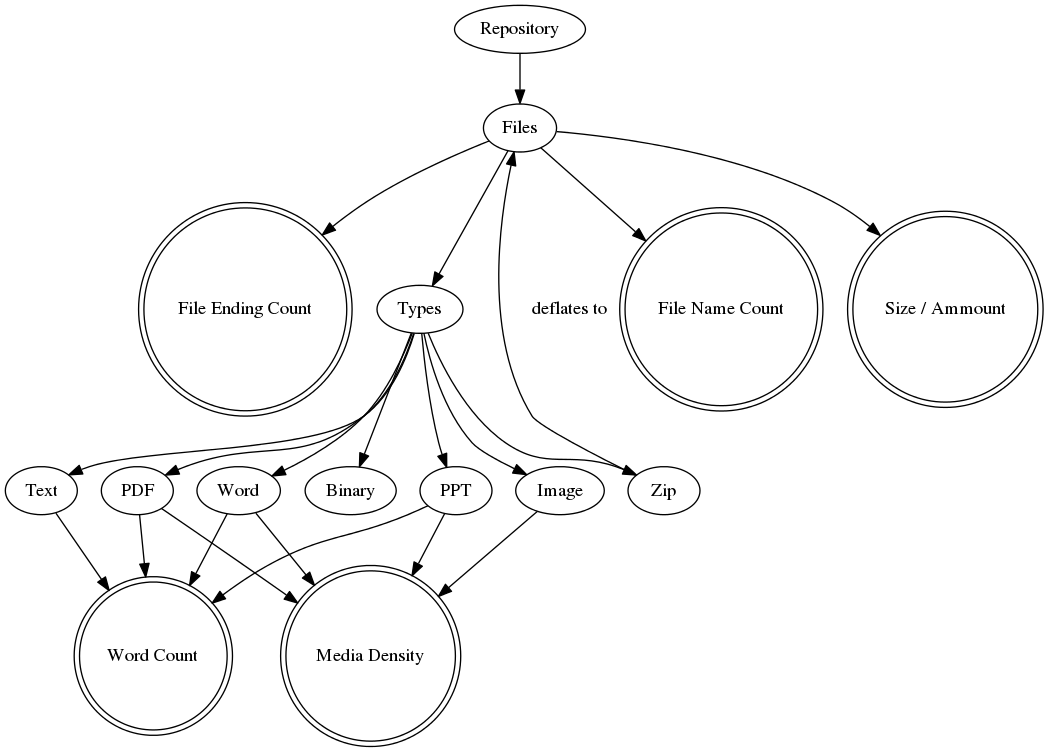
\includegraphics[scale = 0.45]{images/graph1387.png}}
		\caption{Dictionary calculation visualized}
	\end{figure}
	The entries with a double circle represent our features.
	
	In the following sections we will explain our decision why we chose these features and dismissed others.
	
	\subsubsection{Word Count}
	The Word Count represents our most important feature. It is defined as the occurrence of each word contained in any text across the whole repository. This includes all readable text files, and text contained in PDF, Word and Powerpoint files. The contents of the readme file count 10 times as much since it usually contains the most important information. 
	We chose this feature because the Word Count represents a wide range of the repository’s content. At this point we should keep in mind that the information noise especially for the word count is immense. 
	
	\subsubsection{File Ending Count}
	
	The File Ending Count is defined as the occurrence of different file endings in the whole repository. We chose this feature because file endings reflect the use of different programming languages and other file formats in the best possible way.
	
	\subsubsection{Filename Count}
	
	Just like the File Ending Count, the Filename Count is defined as the occurrence of different file and folder names in the whole repository.
	We chose this feature because there are several key files and folders which are in favor of a specific category.        
	
	\subsubsection{Media Density}
	
	The Media Density describes the ratio between the total count of media files and the total word count included inside the Word Count. Media files contained inside PDF, Word, Zip and Powerpoint files are counted as well. We chose this feature because there are specific repository categories that tend to use more or less media files.
	
	\subsubsection{Average File Size}
	This feature is mostly used to detect the ratio between file number and its size. This feature correlates with the Media Density but it is mainly used to detect big crowed files. This would rather indicate a DOC or EDU class than the OTHER or DEV class.
	
	\subsubsection{Number Density}
	At first we did not thought about this feature. But as we build our dictionaries \hyperref[sec: dictionary]{(Chapter 4)} we noticed that occurrences of numbers varies greatly between the classes. Thus we decided to use a feature to merge every number: the Number Density.
	
	\subsubsection{Stared to Subscribed Ratio}
	This value mainly addresses the development class as the probability of a DEV repository to be subscribed and not just liked is (in a selected sample) in general higher. We decided to not use this value because it is too vague and the absolute numbers of stars and subscribers is rather small so that tiny natural deviations could result into a completely other ratio and therefore to a false interpretation.
	
	\subsubsection{Commit Messages}
	The use of Commit Messages and Commits in general was slightly problematic. While we seriously thought about using this as a feature we realized that Commit Messages are too variable. This would be like trying to interpret the interpretation of information so the possibility to classify repository wrongly based on the messages is not as small as we wish it to be.
	
	
	Furthermore available data provided by a simple web browser are immense. Since we need to know the possiblity of accessing these informations we took a look into the Github API instead. This resulted in a major problem: The Github API only allows 60 unauthenticated requests per hour and 5000 for authenticated ones(1). Even if we take into count that only authenticated requests are used, which would require each user to own a Github account, 5000 requests per hour are not enough to analyze hundreds of repositories per hour. There are repositories with over 500.000 Commits and a single Github request returns only the first 500. So we would need 1000 requests for a single repository just to get all of the Commits.
	
	\subsubsection{E-Mail of repository owner}
	This feature is problematic. We thought about searching for an edu substring in the email but we could not find a correlation with the EDU class. Apart from this we could not think of any part in an e-mail which could be relevant.
	
	
	
	
	
	\section{Gathering selected features from Github}
	
	\subsection{Gathering the Repository’s content from Github}
	
	\subsubsection{Choosing the content acquiring method}
	
	To gather the repository’s contents one would normally request the File Tree which represents a list of all available files including their size, their name and their download link. If a file should be further analyzed in detail, one would get its content via File Tree’s download link.\footnote{\url{	https://developer.github.com/v3/git/trees/get-a-tree-recursively}}
	
	The main issue using this method is the previously mentioned rate limit of Github’s API. Requesting each file that should be analyzed individually results in hundreds of requests per repository.
	So instead of requesting each file on its own, there is the option to grab the entire content as “zipball”. On the one hand this results in only one request per repository and the content is already compressed, on the other hand we may grab files that we are not going to analyze at all. 
	Additionally we discovered that the zipball requests are not limited to 60 unauthenticated requests per hour. This makes grabbing the “zipball” superior to requesting the file tree. This way our classifier does not need any form of authentication, our classification performance is therefore only limited to our network bandwidth and the hardware of the operating system.
	
	\subsubsection{ Grabbing the “zipball”}
	
	
	The resulting downstream of the grabbed "zipball"\footnote{Request: \url{https://api.github.com/repos/username/repositoryname/zipball}} is inflated on the fly into multiple virtual files. A virtual file describes a file that is not written onto hard disk, instead it is kept inside the classifier’s heap. This results in a huge RAM usage but allows much faster processing of the gathered files.
	
	\subsection{Categorizing Files}
	
	In the next step all virtual files are categorized into the following eight different categories: Zip, PDF, Word, PowerPoint, Text, Binary, Image and Folder. The category in which a file belongs is determined by a fixed procedure. 
	At the beginning it is checked if this is a folder. If it is not we use arimus’s jmimemagic libary https://github.com/arimus/jmimemagic to get the file’s Internet Media Type (MIME-Type). If the MIME-Type can’t be parsed from the file, there is still a chance that the investigated file could be a readable text file. To avoid missing such files we use an additional method to guess whether or not the file is a readable text file. The method basically calculates the ratio between the amount of ascii bytes and other bytes. If the ratio of non ascii bytes is greater than 5\% we assume the file is not a readable text file. Nevertheless we neither rely on this method nor on the MIME-Type. Instead we use both in combination with the file’s extension, to make the final decision in which category a file belongs. If a file falls into either the Binary or the Image category its content stored inside the heap gets released, since we can not analyze these files further.
	
	\subsection{Inflating the Filelist}
	
	The Zip Category contains all types of archives that are inflatable. We think that a lot of information can be hidden inside the archives, we inflate them, and they undergo the same procedure like the “zipball”. The recursive depth of this method is one, so archives inside archive files that are inside zip files are not analyzed. The reason behind this decision is the resulting performance impact as well as the lacking relevance of files gathered by a deeper recursion for the repository’s type.
	
	\subsection{Getting Word Count}
	
	\subsubsection{ Access non readable files that contain text}
	To extract the Word Count out of the inflated file list, we need to get access to the text contained in the non readable text files. To extract it out of PDF files we use Apache’s PDFBox library inside a simple wrapper class, which allows us to extract the raw unformatted text out of pdf files. For the Microsoft’s PowerPoint and Word files we use Apache’s POI library in a similar way.
	To avoid opening any file twice we also extract the amount of Media Files inside the analyzed files. 
	
	
	
	\subsubsection{Formatting the raw text}
	To get as many matches as possible, we normalize the raw text. First of all we remove all hyphens followed by a line break. This way we can restore any word that was splitted due to a line break. Afterwards all line breaks are replaced with a whitespace. This is needed because the Scanner we use to parse single words from the normalized text uses a whitespace as delimiter. In the next step we replace all non ascii letters with ascii ones. This would convert the following String “äèôãç” to “aeoac”. This step is needed because in the next step all non ascii and other special characters are being removed.
	
	\subsection{Counting Words}
	To count the words gathered by the Scanner we use a HashMap that takes a String as key and stores an Integer as its value. This allows us to count the occurrence of all words with O(n) complexity. For further performance improvement we formatted the raw text and counted the words in and separated them into two different threads.
	
	\subsection{Calculate the Fileextension and Name Count}
	
	To calculate the File Extension and Name Count we iterate through the inflated file-list using the same counting method as for the Word Count with a few modifications. For files without an extension we defined a unique custom extension named “filehasnoending”.
	File names get normalized and their path inside the folder structure gets removed.
	
	
	\section{Removing irrelevant information from selected features}
	\label{sec: dictionary}
	\subsection{Algorithm to create Dictionaries}
	Especially the features \textit{File Ending Count}, \textit{Word Count} and\textit{ Filename Count} still consist of information noise as every repository could contain words that are unique to every other repository and are therefore not relevant for the classification. Then again some words could be in almost every repository but their occurrence does not differentiate between the classes in a considerable margin. Due to the rising complexity of a neural network for every input added to it, one should try to find a balance between the number of words and the relevance of a word. We decided to create a dictionary for each of the mentioned three features that contains every relevant word for classification.
	The question arises how to choose the words for the dictionaries. Therefore we created an algorithm.\\
	
	
	The algorithm takes classified repositories, we choose to use our Training Datasets \hyperref[src:Repositories]{(Chapter 8)}.
	In the first step the intersection with a threshold $p$ of words between repositories of the same class is calculated for each repository class. The threshold $p$ is used to define the minimum ratio between repositories that contain the word and the total number of repositories in the class. 
	This step is used to filter words that are too unique.
	
	
	In the next step the ratio between the occurrence probability of a remaining word in a class and the average occurrence of a word over \textit{all} repositories is calculated for every word and class. We will thus sort the seven (in case we have seven classes) lists from large to small. This step is used to find the words with the highest deviation from the average occurrence and therefore helps to classify a repository. Combined with the first step we thus selected words that exist in many repositories. Moreover their occurrence probability is highly dependent on the class of the repository.
	Our dictionary is then created by adding the first $q$ words of a list of each class to a set (because words can exists in multiple lists).
	\begin{figure}[H]
		\subfigure{\label{konfiguration}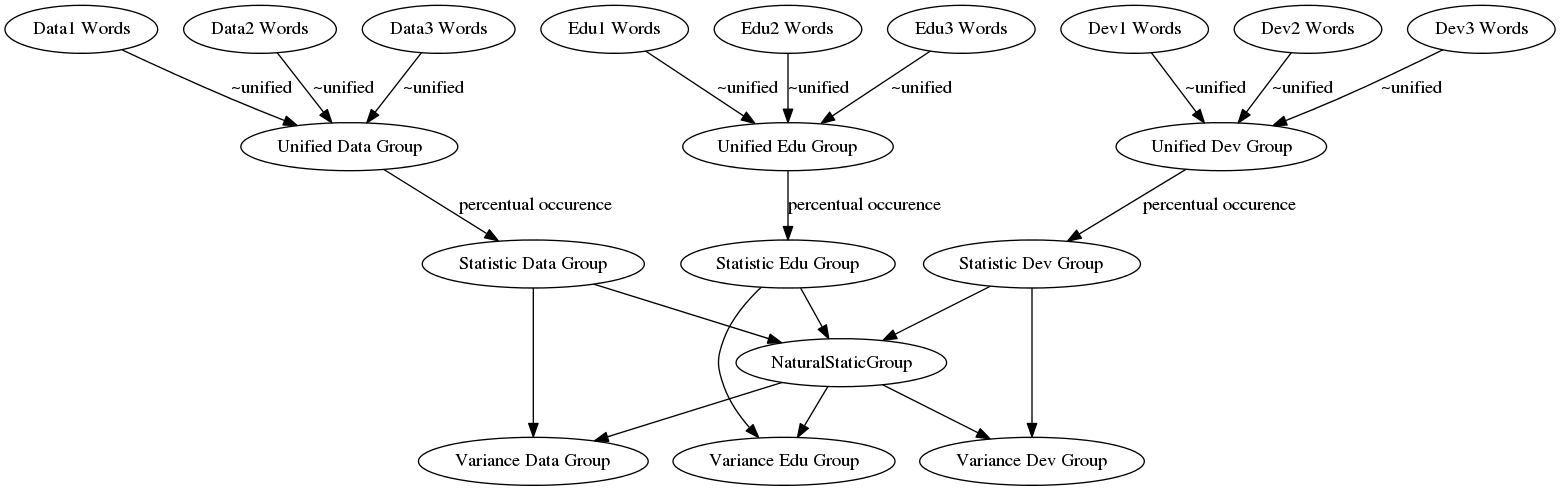
\includegraphics[width = 1.1\textwidth, height = 200px]{images/dictionary.png}}
		\caption{Dictionary calculation visualized with three classes}
	\end{figure}
	
	\subsection{Created Dictionaries} 
	So the next important step is to choose $p$ and $q$. At this point we should add that we did not try to choose the dictionaries by just watching over the selected words.
	We rather tried to use the information we know about the words and their deviation to generate them. We tried to calculate the optimum between number of words and deviation as well as occurrence probability (the initial created dictionaries are still open to change in the optimization step (\hyperref[src:optimizing]{Chapter 6}).
	These are the three dictionaries with less information noise we used after the optimiziation phase \hyperref{src:optimizing}{Chapter 6}:
	\\
	
	\paragraph{File Ending}
	iml ps cls tmp orig graffle eps large art sty hdr cproject woff2 hs launch rhistory tga eot woff gitattributes am pyx prototxt cu groovy prefs ds store xsd project less mf pri mm erl mat hpp dtd jar r ui glsl ru out pem lock qrc kml ttf svg in scss bin s otf iwa yaml d qdoc npy coffee rdx rdb rdata f pl tex qml conf map jpeg markdown properties rmd cache pod gitignore cs sh pro keep php data rst gif erb m csv npmignore css txt cpp yml c pdf java h rb py html class png filehasnoending xml jpg md js json 
	
	\paragraph{File Name}
	session10 cheat pykcharts session2 district percentage session1 sheet india united south america git day glyphicons bar house country rock sec2 men secret collection pradesh buttons sec3 gear francisco black sec1 master light line lord top t is fragment slide twitter img vs nfl theme v1 my king san math template pdf france as r o time locale final changes for small linux ssl california 2x new gui i x ui plot game bg exercises c icon slides resources view repository root info java sample org it pom in topo init xml basic error controller types array on bootstrap db build all b and resource to parser js html regular min application css p app source config s makefile world modules src example no map the a unnamed chunk utils node of data lib main test license package readme index homework assignment 
	
	\paragraph{Words}
	multipolygon engtype varname censuscode brk pradesh adm0 cen district wb nm python chart os cd a3 dt arcs polygon a2 iso durch nr bis einer pra ber def eine bei zur install import sind werden info nicht auf das dem nba abs properties im attr paper gender joseph ui william san ist tate zu returns none me insurance mm art mit sf den nach element von uk txt qt observed images st div app result list ownership sector left profile oder turner solo hour fa any percent sizes lb required events span views vt sic tags const get timestamp california uri num segment hispanic version style promise void values male path des original license www years comments set err key size white state require u else jpg from female und l county error g source o private callback vn title url length it false as that no y h on with x m pc null file class string node object album all an true be by js start options children data org username d net https com v value type der t die end text http not s f int b or image column var row of line and for in is e return r name w to this function xml if c n id the rd a i homework assignment 
	
	\section{Building the Prediction Model}
	
	\subsection{Choosing a prediction Model}
	There are many different approaches to the problem. A static algorithm to classify repositories is rather impractical because the parameters of our classify function would be strongly influenced by our interpretation of how we weight features for each class. However we quickly noticed that the complexity is very high so that a normal algorithm would limit the aspects which possibly needed to be considered. The problem is non-linear and through the static analysis we would lose the possibility to freely improve or change the classifier. As the software and use-case market of Github rises, the possible need of further classes could arise.
	
	
	To ensure a classifier who is as dynamic and as extensible as possible we choose to use some form of machine learning.
	The problem which needs to be solved by the Prediction Model is a classification problem: As input we have a fixed number of values for selected features  and as an output the class to which the values fit the most. As a result of this it was pretty clear to us that a supervised learning method would be optimal.
	
	
	In the next step we thought about the pro- and contra arguments of non-parametic and parametic learning.
	Gaussian-Process-Models for example could theoretically be used, as one does not need to specify a fixed number of parameters and therefore be non-parametic. 
	The main problem with Gaussian-Process-Models is that they scale rather poorly with a complexity of $O(n^{3})$ \cite{DukeUniversity}. Moreover if we keep the huge dimension of repository datasets in mind and thus the possible complexity of the classifier function, our choice will lead us to a parametric neural network. A neural network combines every important aspect from above and is furthermore capable of performing well in the presence of imprecise and especially noisy data.
	
	\subsection{Our Neural Network Model}
	First of all it is not needed to consider temporal behavior for our selected features. We do not need to save an internal state (if we had used a sequence of Commits this could have been otherwise). It should be fully sufficient to use a Feed-forward neural network.
	
	As for a neural network with supervised learning we choose that a Multilayer perceptron(MLP) with one hidden Layer would be sufficient for our classification problem. We already mentioned that our classification problem is not linear. Hence at least one hidden Layer is required to solve the problem. Furthermore we know that this MLP can approximate any bounded continuous function with arbitrary precision \cite{ApproximateAnyFunction}. From this follows that the probability to solve our problem with one hidden Layer is high.
	The usage of a linear activation function would result in a MLP with a set of possible functions to be equivalent to those of a normal input-output perceptron. Therefore we needed to use a nonlinear activation function. We thus decided to use a sigmoid function. 
	
	For the training we used Backpropagation as expected for a MLP. To reduce the chance to be stuck in a local minimum we used inertia so that the previous change will influence the weight adjustment in the current iteration.
	
	The neuron count for the output-layer is set to the number of different classes into which we want to classify the input. So for our Neural Network we used seven output neurons.
	
	Our input neurons count equals to the sum of the length of every dictionary plus all relevant ratios of our selected features.
	
	\subsection{Formating and further preprocessing of Features to fit into the Neural Network}
	We tried to find the perfect balance in preprocessing so that on the one hand the network does not need to learn obvious relations between features and on the other hand it does not lose possible relations by too much preprocessing.
	
	
	To format the input for the neuron we will iterate through every word in a dictionary of a type. The ratio between the relative occurence of the word for this type and the occurence value stored in the dictionary is calculated. Effectively this ratio is equal to the deviation of the relative word occurrence for the considered type. In case the relative occurrence of a word ending is higher then the occurrence in the dictionary it will result into a value $> 1$. Hence there is still the necessity of a normalization process - for the dictionary deviation as well as for the ratios.
	
	
	There are several possibilities to normalize the input. In our case it is important that the input is distinct. Furthermore standard normalize procedures are using a maximum and minimum value. The problem is that it is not possible to define an upper bound for the inputs because a test-input could always exceed the previous bound and therefore the attribute of distinction is contradicted in case the input should still be normalized (new Max value could lead to values to have the exact same value as a value with an old bound). Nonetheless we tried the different normalization procedures of min-max normalization and standardization but the results were rather disappointing so we will not go deeper into this.
	
	
	Therefore we decided to use a logistic function to normalize our data. A logistic function is monotonically increasing and thus for every value distinct. Depending whether we use a sigmoid or tanh function we will construct the logistic function in a way that the upper bound is 1 and the lower bound respectively 0 or -1 in case of the tanh. 
	We can then use a constant of proportionality to optimize the distribution of the values:
	
	$f(x) = 2 * \frac{1}{1 + e^{-k(x-k)}} -1$
	
	To support the understanding of our normalization technique we will plot our function for $k \in \{0.03, 1, 5\}$.\\
	\begin{figure}[H]
		\subfigure{\label{konfiguration}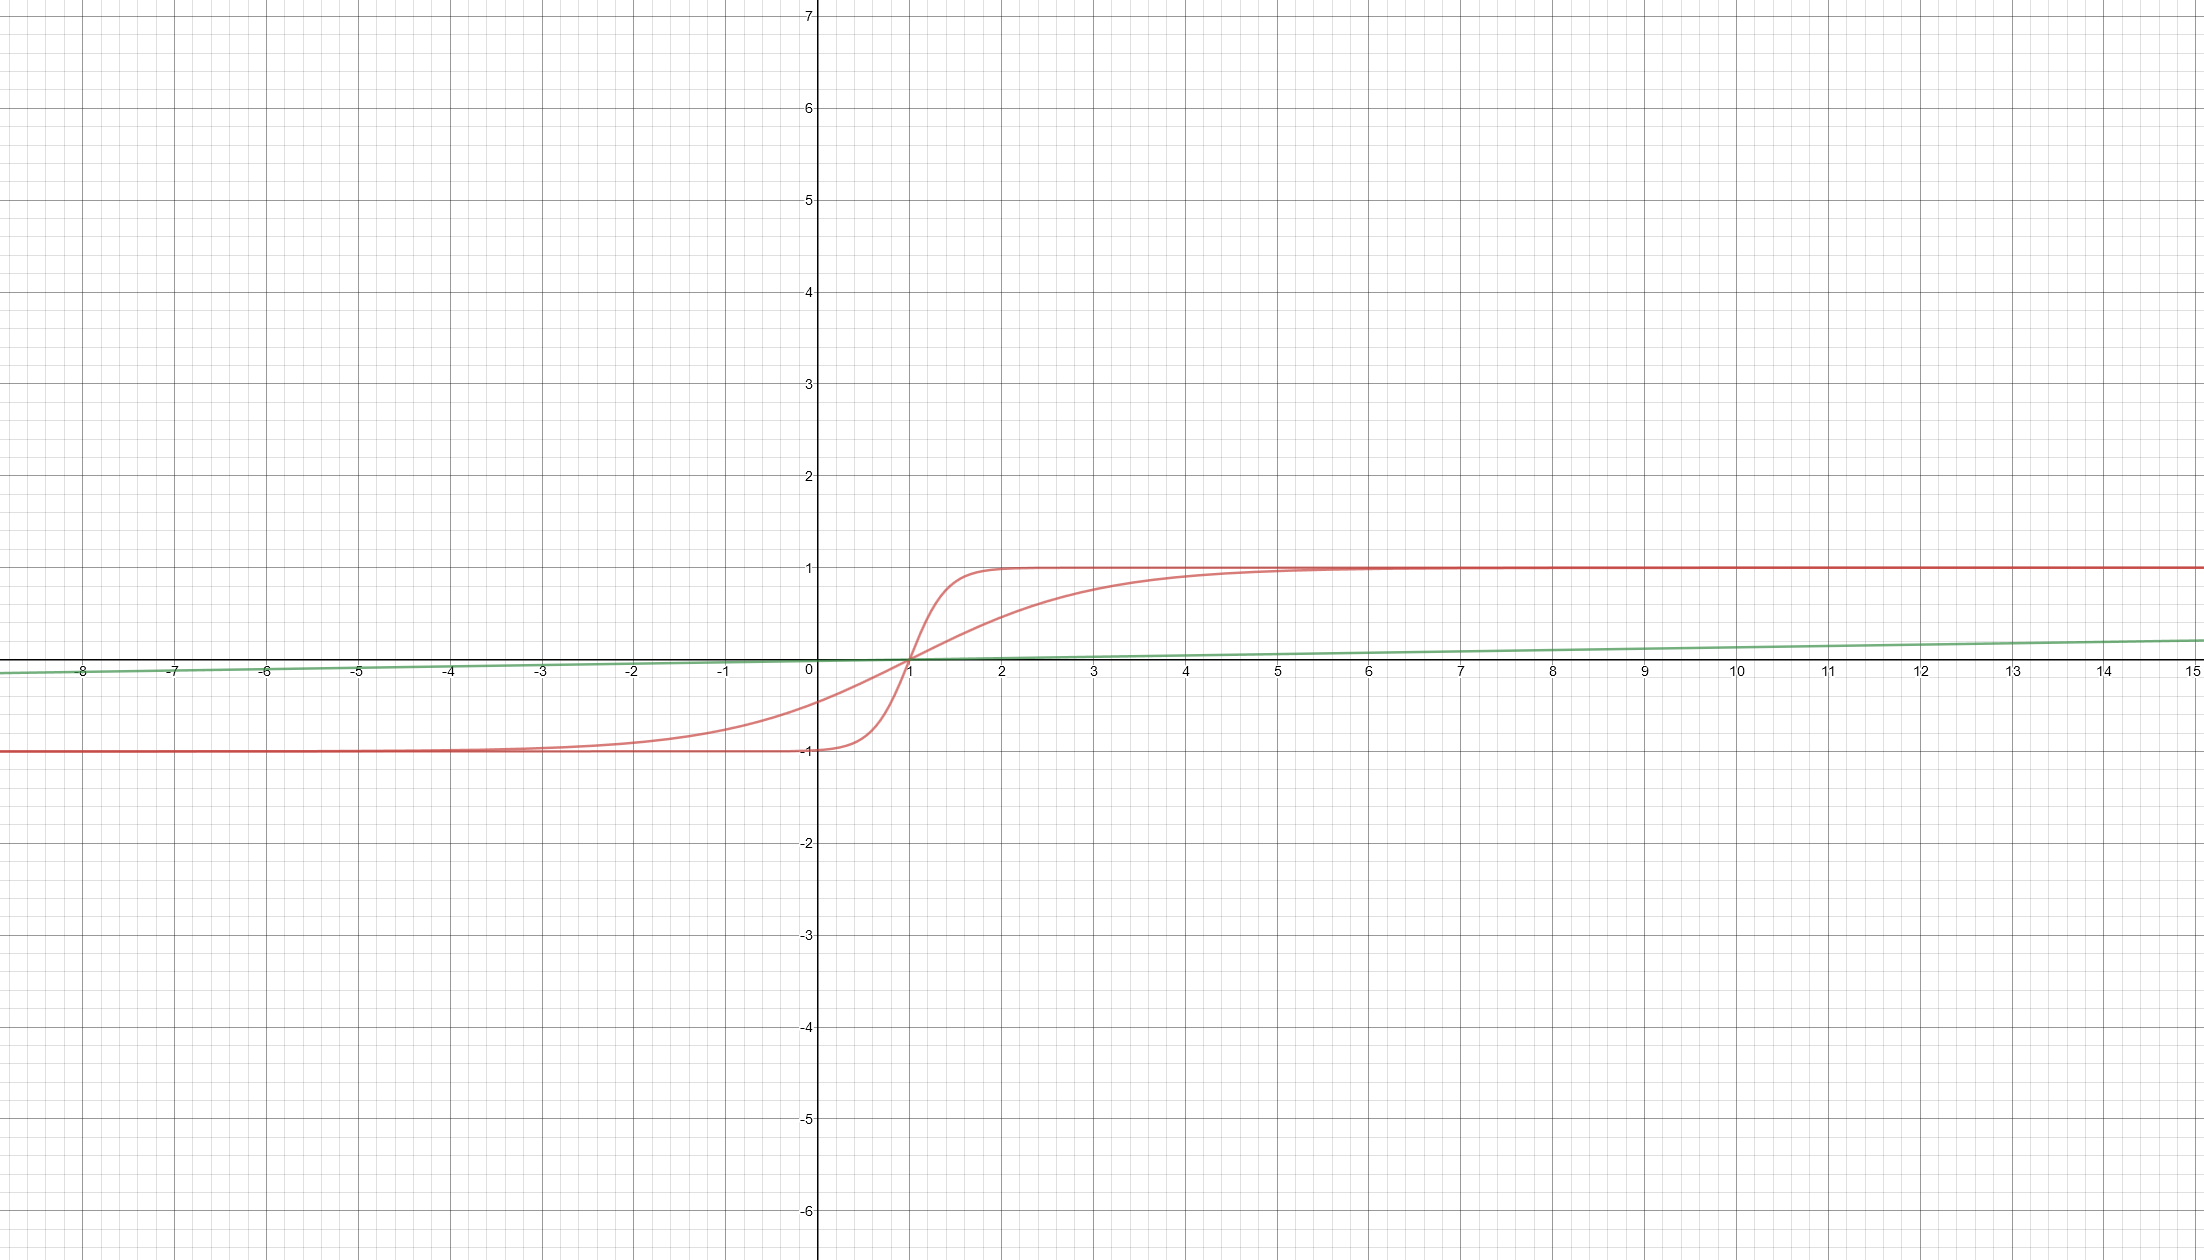
\includegraphics[scale = 0.2]{images/logistic.png}}
		\caption{k = 0.03 in green, k = 1 in bright red, k = 5 in red}
	\end{figure}
	
	The normalization process will take place for every dictionary and ratio but they all have to define their own proportional constant.
	Every value is stored as a double and the index position of every feature is static.
	
	
	
	
	
	\subsection{Data Sets and Training}
	Besides the labeled repositories in the challenge description we used most\hyperref[src:TrainingRepositories]{(Chapter 8)} of the the additional additional repositories \hyperref[src:Repositories]{(Chapter 8)} provided by a participating team in the official Github repository of the InformatiCup 2017 as training repositories (although you cannot read it: a big thank you at this point!). We have to admit that even as a human being the classification is not as clear as we thought it would be. Sometimes we were not sure if the labeling of the data sets we used were correct and we realized that many repositories overlap with different classes. It is not always objectively clear to which repository it fits more. In this case the repositories were labeled by personal preference and estimation. Therefore the learning of our network is influenced by personal decisions as it uses the labels.
	
	Since we are using backpropagation after each iteration, the actual output of the network is compared to the desired output. Using the euclidean distance leads us to an error value. The Training continues until this error value is below a manual set value.
	
	
	
	\section{Optimizing our Neural Network }
	\label{src:optimizing}
	A potentially very time consuming task is to optimize the network. We divided the possible optimizing parameters into three classes. Firstly we need to optimize the training. Besides changing the inertia and learning rate it is far more important to take care of the error value of the neural network. A minimum max-error value far too low could result into overfitting the neural network to the repositories of the training phase. Then again a minimum max-error value that is too high would result into a very unstable and an underfit network. 
	
	
	The second category would be optimizing the features selected in the beginning. We have to consider that our selected features are not as optimal as expected.
	Lastly we need to optimize the neural network itself. This includes the hidden layer as well as the preprocessing step of normalizing the values.\\
	For testing we used the Test Repositories given by the Challenge Description. To prevent an overfitting on the Test repositories we decided to use further ones provided by the additional Dataset for testing. We used 36 more Repositories (6 per class) so that we tested our neural network on 67 Repositories \hyperref[src:TestRepositories]{(Chapter 8)}. While intuitively classifying these repositories \hyperref[src:ClassifyTestRepositories]{(Chapter 8)} we noticed again that some repositories could be classified in multiple classes. It is hard to say to which it fits the most. 
	
	
	 We thought about different methods for testing. Known procedures like k-fold cross validation do not have benefits in our case because in our opinion the dataset is not big enough for this. There is a natural deviation of results in each change of a parameter and it is not easy to tell whether this change has been random or has really improved the network. The rather small datasets we would obtain for k-fold cross validation would increase this problem while reducing the possible overfitting. Nonetheless we decided to stay with our fixed 67 repositories.
	 
	We used the accuracy (ratio of overall correct classified repositories to the total number of repositories) to evaluate our results. We chose it because besides the OTHER class every class is nearly similarly important and therefore every correctly classified value is nearly equally important.
	We decided to change the parameter values of neurons in hidden layers, the values $p$ and $q$ for the dictionary, the weight of the Readme words, the max-error value and the proportional constants $k_{wordDictionary}, k_{fileName}, k_{fileEnding}, k_{ratios}$ for our defined logistic function.
	We firstly changed the $k$ values as they are not as variable as the other values. We need to find a value so that the function distributes the input values even. This could be done by calculating the average distance between the values.
	The next step was used to modify the max-error value.
		\begin{figure}[H]
			\subfigure{\label{konfiguration}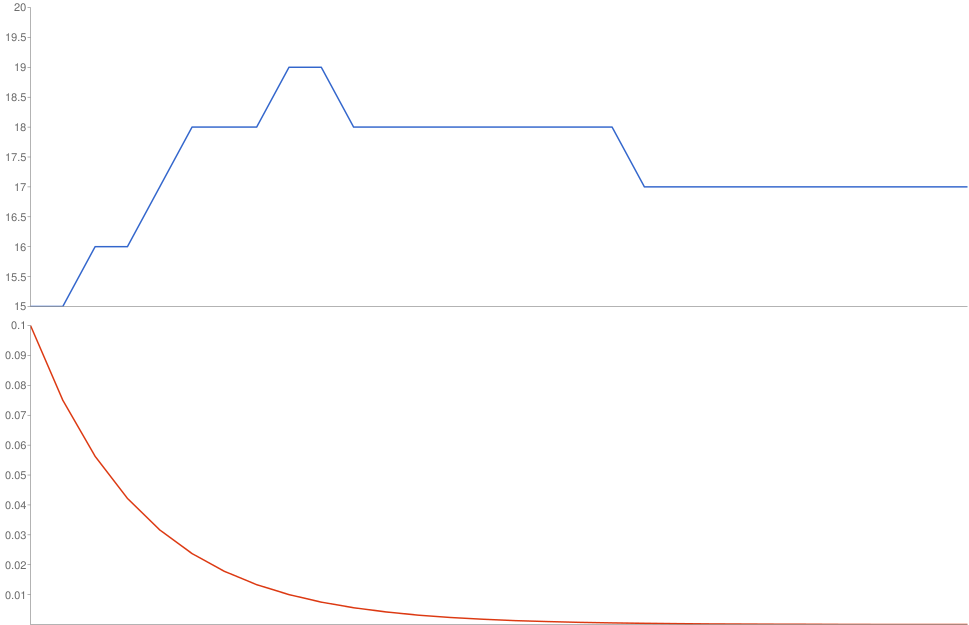
\includegraphics[scale = 0.45]{images/messung1.png}}
			\caption{red graph is the max-error(range from $0.1$ to $2381094536 * 10^{-5}$) and the blue graph are the correctly classified repositories}
		\end{figure}
		
	We continued optimizing our network with changing the number of Neurons in our hidden layer.
		\begin{figure}[H]
			\subfigure{\label{konfiguration}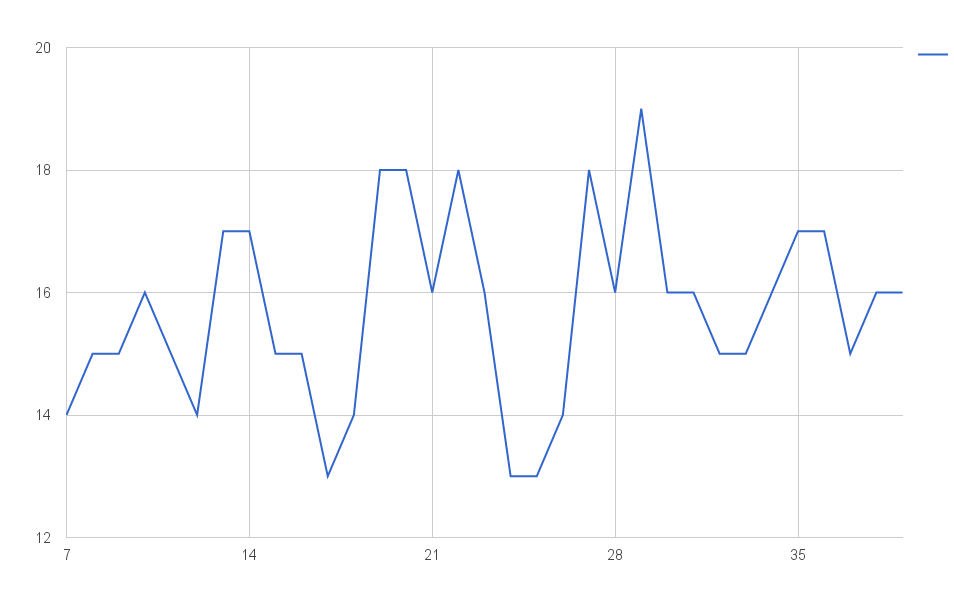
\includegraphics[scale = 0.45]{images/messung2.png}}
			\caption{number of hidden Layer on the x-Axis and correctly classified repositoried on the y-Axis}
		\end{figure}
	 

	As you can see the results are oscillating to a lesser extent. The optimization process from this point on was not as easy. Taking the optimal result of each parameter while keeping the others constant does not necessarily lead to the best result. In fact it is possible that the optimal results are manipulating each other so that the overall result is even worse. 
	Thus we needed to try out the different parameters while using predictions and guesses. At this point we will not talk further about non optimal results (\hyperref[src:recordingsOfResults]{Chapter 10: Results}). 
	The parameter values for our optimal result are:\\
	 hidden Layer = 39, max-error = 0.01 $p$ =  and $q$ = for the dictionary, the weight of the Readme words =  $k_{wordDictionary} = 0.45599, k_{fileName} = 3.206 , k_{fileEnding}= 6.14125, k_{ratios} = 0.001$.
	
	\section{Validation of created Classifier}
	As requested by the challenge description we created a boolean matrix for comparing the results of our neural network to our own classification. The order is identical to these of the test-repositories \\
	
	$\begin{pmatrix}
		1 & Intuitive & network & \cap\\
		2 &  HW & HW  & 1 \\
		3 & DEV & DOCS & 0 \\
		4 & EDU & EDU & 1 \\
		5 & EDU & EDU & 1 \\
		6 & DEV & DEV & 1 \\
		7 & WEB & WEB & 1 \\
		8 & DEV & DEV & 1 \\
		9 & DOCS & OTHER & 0 \\
		10 & EDU & DEV & 0 \\
		11 & DOCS & DOCS & 1 \\
		12 & DEV & OTHER & 0 \\
		13 & HW & DOCS & 0 \\
		14 & DEV & WEB & 0 \\
		15 & DEV & DEV & 1 \\
		16 & OTHER & OTHER & 1 \\
		17 & DEV & WEB & 0 \\
		18 & DOCS & DEV & 0 \\
		19 & DEV & DEV & 1 \\
		20 & DOCS & DEV & 0 \\
		21 & WEB & WEB & 1 \\
		22 & DEV & DEV & 1 \\
		23 & EDU & EDU & 1 \\
		24 & EDU & HW & 0\\
		25 & DATA & DATA & 1 \\
		26 & DATA & DATA & 1 \\
		27 & DEV & DATA & 0 \\
		28 & DATA & DEV & 0 \\
		29 & DEV & DEV & 1 \\
		30 & WEB & WEB & 1 \\
		31 & EDU &  WEB& 0\\
		32 & EDU & OTHER & 0 \\
	\end{pmatrix}$
	\\
	\newpage	
	For the next step we calculated the precision and recall as defined.
	\\
	
		$\begin{pmatrix}
		    & Recall & Precision \\
		   \hline
		DEV & 0.55 & 0.6\\
		 WEB& 1.0 & 0.5 \\
		 OTHER& 1.0 & 0.25 \\
		 ED U& 0.43 & 1.0 \\
		  DATA & 0.67 & 0.67 \\
		  HW& 0.5 & 0.5 \\
		\end{pmatrix}$
	\\
	\\
	First of all the results are disappointing, nonetheless it is possible to see many things and problems in our network through this matrix. A highly noticeable issue is that every repository of the class OTHER was identified but many wrong repositories were also put in this class. Therefore it seems that our classifier trains a little bit too hard on OTHER repositories. We have several reasons why this could have been the case: As we mentioned earlier we tested and trained our network with a rather balanced repository set. Therefore OTHER has always more or less the same weight as the other repositories. However our own classification of the test repository only classifies one out of 31 repositories as OTHER and therefore just 22\% of the expected occurrence. Moreover this result somehow reflects our decision to evaluate the results with the accuracy.\cite{EvaluateNetwork}
	
	
	Furthermore we noticed that the influence of the WEB class is too high. 50\% are wrongly classified while the recall is at 100\%. The selected features are seemingly strong indicators for WEB repositories however they are not exclusively enough.
	
	
	With this information in mind we think our repository would work very good on following three repositories:\\
	\url{https://github.com/Raldir/HomeworkNr3}\\
	\url{https://github.com/alanerzhao/doc}\\
	\url{https://github.com/jailecoeu/wechat}\\
	
	
	 The importance of yield and precision depends on the use-case. A search function with a filter for each category for example might rather have a high recall in case the classes are evenly divided. The importance lies in finding as many repositories of the right type as possible, some outliers are not that big of a problem. Equal to the Test-repositories the distribution of the classes would not necessarily be balanced in a real case scenario. Under this assumption it would be possible that we are searching for a class which occurs rather rarely on Github then it is far more important to gain a high precision while holding the recall stable. If for instance a repository type occurred 0.1\% on Github and there were 100.000.000 repositories in total, the difficulty on obtaining a specific precision would be a lot higher than on a balanced classification problem. Therefore it is very important to optimize the precision in these cases.
	
	
	In case the number of considered repositories is low then a higher recall would be preferable because it would be more important to find the desired repository in the selected number. Then again the use case here is a different one from the above. The focus would lie on looking through the own repositories and searching for a special repository taken for class. It would be far more important to find the desired repository even though classifying some wrongly. Having a high precision but missing repositories at the same time would not be satisfactory for this use-case.
	
	
	All in all we would say that a high precision is more desirable for the realistic and reasonable use-case of the classifier. In our opinion a classifier benefits the most when the total number of repositories is high because it would not be as easy for a human to filter the desired repositories. It is possible to apply a classifier on a small number of repositories but the benefit would be not as big as most of the time it is known to oneself what is located in the own repositories.
	To underline the importance of a high precision we searched for possible indicators for imbalanced classes (high variance overall for class occurrence in set of repositories).
	
	
	\section{Extensions}
		We also created a visualization tool for visualizing the process of gathering the data, preprocessing them and till the final classification of a repository finished. We tried to do it in a very intuitive way while still fulfill a functionality.
		
		The dictionary creation process for example always shows the 65 words with the highest occurrence.
	
	\newpage
	
	\begin{thebibliography}{xxxxxx}
		\bibitem [1] {DukeUniversity} David P. Williams "Gaussian Processes" (2006) \url{http://people.ee.duke.edu/~lcarin/David1.27.06.pdf}
		\bibitem [2] {ApproximateAnyFunction}  Cybenko., G. (1989) "Approximations by superpositions of sigmoidal functions", Mathematics of Control, Signals, and Systems \url{http://deeplearning.cs.cmu.edu/pdfs/Cybenko.pdf}
		\bibitem[3] {EvaluateNetwork} Marina Sokolova, Guy Lapalme "A systematic analysis of performance measures for classification tasks" \url{http://rali.iro.umontreal.ca/rali/sites/default/files/publis/SokolovaLapalme-JIPM09.pdf}
	
	\end{thebibliography}
	
	
	\section{Source Code, used external Libraries and Repositories}
	\paragraph{Source Code}
	Github: \url{https://github.com/Crigges/InformatiCup2017}\\
	\paragraph{Repository Dataset}
	\label{src:Repositories}
	\url{https://github.com/InformatiCup/InformatiCup2017/tree/master/additional_data_sets}	\\
	
	\label{src:TrainingRepositories}
	\paragraph{Training Repositories}
	Exact repositories used for training can can be found on the relative path to the root folder ./assets/TrainingRepositoriesSet2.txt.
	
	\label{src:TestRepositories}
	\paragraph{Test Repositories}
	Every test-repository can can be found on the relative path to the root folder ./assets/CombinedTestRepositories.txt.
	
	\paragraph{Intuitive Classification}
	\label{src:ClassifyTestRepositories}
	Intuitive classification of the repositories can can be found on the relative path to the root folder ./assets/TestRepositorys.txt.
	
	\label{src:recordingsOfResults}
	\paragraph{Recording of Results}
	Some recordings of our (non optimal) results are located in the doc folder: SampleResults.xlsx
	
	
\end{document}



